\section{Requirements Captured}
The following are requirement divided into functional and non-functional requirement which where collected after consulting with the client.
\subsection*{Functionality requirements}
The list of the requirements for the application where as follows:
\newline\textbf{Functional Requirements}
\begin{itemize}
	\item Rendering of the map on the user screen
	\item Have signal strength indicators on the map. These should be updated on a real-time basis.
	\item Save signal strength on the database for a specific location.
	\item Zoom in and zoom out of the campus map
\end{itemize}
\textbf{Non-Functional Requirements}
\begin{itemize}
	\item Real-time receiving of data being updated in the database.
	\item Speed up on the rendering of the areas and their strengths on the map.
\end{itemize}



The next section deals with the analysis of your system. Cover the
functional, non-functional and usability requirements. This is where
you present your use case narratives and diagrams. 

Discuss the major analysis artefacts that you produced. We will expect
you to produce at least one overall description of the architecture
used in your system as a diagram, either here or below (see Section
\ref{ss:design-overview}). You may also want to include an analysis
class hierarchy diagram.

\subsection{Design Overview}
\label{ss:design-overview}
\paragraph{}This Section gives an overview of the system which entails showing how the system interacts with other systems in delivery of functionality to the user and introduce the basic functionality expected from the System,It will also describe what type of stakeholders will interact with the system and what functionality each should expect,finally explain the assumptions and constraints for the system 

\paragraph{}They are mainly Two ways users can interact with the System that is through a mobile Application(Android Only) and Web Application.

\paragraph{}Mobile Application will need to communicate with the phone's GPS system so as to obtain a user's Location.The functionality provided by GPS is crucial as it pinpoints exactly which WLAN Zone data is collected and ensures accurate aggregate Data is displayed on each WLAN zone.

\paragraph{}Wifi Manager will also be needed by the mobile application so as to obtain Wifi Strength of the router to which the mobile phone is connected to a certain point in time,as both the Wifi Strength and Location to which this data is obtained are the main pieces of information driving the System.

\paragraph{}Since this is a data-centric Application,that means data needs to be stored in a database,both Web Application and Mobile Application will communicate with the database but in slightly different ways.Mobile Application will both query and send data to and from the database while
the web Application will be restricted to just querying data from the database for displaying purposes.

\paragraph{}Query Manager is used by both Mobile so as to validate the data collected corresponds to a WLAN zone or else its not written to the database and handles requests of data from both web and Mobile Application to obtain data to display.

\paragraph{}Both Mobile and Web Application use the Mapping System so as to display a Map to the user which includes data collected from the users stored in the database aggregated into different WLAN zones so as to provide appropriate information to the user.

\paragraph{}Cluster System is required by the Mapping System so as to cluster Data points collected which are very close to each other so as to prevent clutter on the Map which is undesirable to the user(Clustering occurs only at high zoom level).  

\paragraph{}Reporting system is used by the Web Client to generate a report which will provide useful information based on the collected data stored in the database.   
 
\begin{figure}
	\centering
	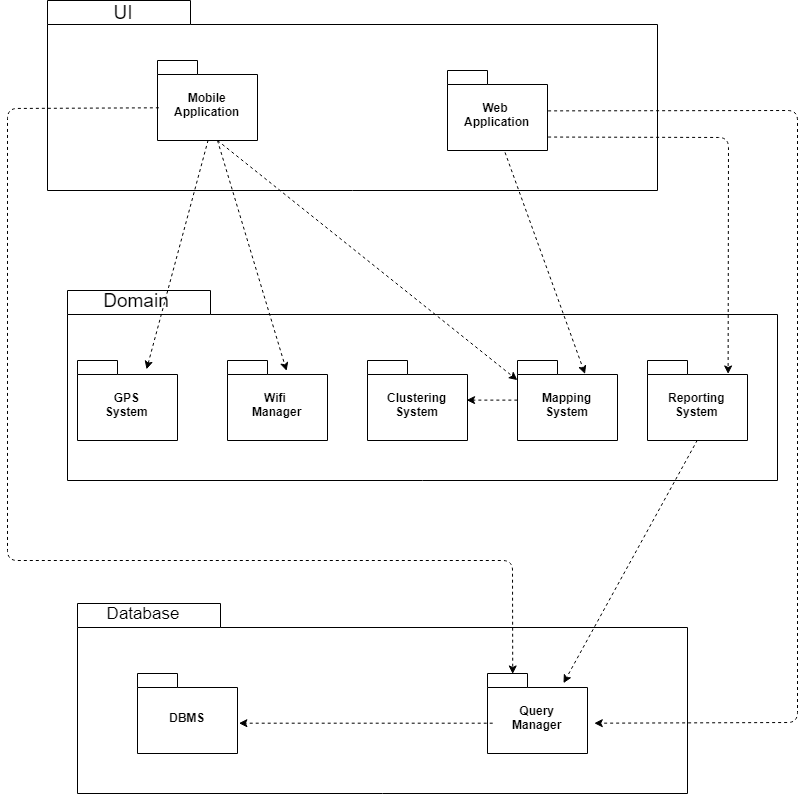
\includegraphics[width=0.7\linewidth]{images/Architecture}
	\caption{Architecture Diagram}
	\label{fig:architecture}
\end{figure}

